\documentclass[8pt]{beamer}
\usetheme{default} % Very simple theme
\usecolortheme{dove} % Minimalist grayscale colors
\setbeamertemplate{navigation symbols}{} % Remove navigation bar

% Define brand-like colors
\definecolor{myblue}{RGB}{0, 102, 204}    % Blue for standard blocks
\definecolor{mygreen}{RGB}{0, 153, 0}     % Green for example blocks
\definecolor{myred}{RGB}{204, 0, 0}       % Red for alert blocks
\definecolor{myorange}{RGB}{255, 128, 0} % For \emph

% Accent color for titles, bullets, etc.
\setbeamercolor{structure}{fg=myblue}

% Block colors
\setbeamercolor{block title}{bg=myblue, fg=white}
\setbeamercolor{block body}{bg=blue!5, fg=black}

\setbeamercolor{exampleblock title}{bg=mygreen, fg=white}
\setbeamercolor{exampleblock body}{bg=green!5, fg=black}

\setbeamercolor{alertblock title}{bg=myred, fg=white}
\setbeamercolor{alertblock body}{bg=red!5, fg=black}
\setbeamercolor{alerted text}{fg=myred}

% Optional: color for \example text
\setbeamercolor{example text}{fg=mygreen}

% Custom emph (orange text instead of italic)
\let\oldemph\emph
\renewcommand{\emph}[1]{\textcolor{myorange}{#1}}


\usepackage{graphicx} % Package for images
\usepackage{amsmath} % Package for images
\graphicspath{{figs/}} % Path to your figures directory
\usepackage{array}  % For better column spacing
\usepackage{caption} % Required for \captionof

% Title Information
\title{STOCHASTIC METHODS IN WATER RESOURCES}
\vspace{25pt}
\subtitle{Unit 2: Hydrological statistics and extremes \\ Lecture 5: Definitions and analysis of extreme values}
\author{Luis Alejandro Morales, Ph.D.}
\institute{Universidad Nacional de Colombia \\ Department of Civil and Agriculture Engineering} %// }
%\date{\today}

\begin{document}

% Title Slide
\begin{frame}
    \titlepage
\end{frame}

%-------
% From Diaz-granados
\section{Definitions and analysis of extreme values}
\subsection{Generalities}
\begin{frame}{Generalities}
    \begin{itemize}
        \item Engineers must deal with different types of risks derived from natural and anthropogenic actions. 
        \item Extremes events, such as \emph{floods}, \emph{droughts} and \emph{landslides} can trigger human, economical and environmental losses. 
        \item This means that civil and environmental  engineering design must consider the occurrence of extremes events, even these seldom arise. 
        \item The analysis of extreme events is made based on historical data, usually recorded at daily time scales, of streamflow, rainfall, water levels, temperature, wind, etc. from where probability distribution of extremes are obtained. 
        \item However, because of the length of  records, usually the number of extreme values is low and  thus the precision of the estimation of the probability distribution decrease.    
    \end{itemize}
\end{frame}

\subsection{Hazard, vulnerability and risk}
\begin{frame}{Hazard, vulnerability and risk}
    Extreme hydrological event triggers  negative effect on economy, environment and population. To understand the these effects is necessary to define the following concepts in the study of extremes. 

    \begin{block}{Hazart ($A$)}
        \alert{Hazard} is the probability that either a natural or anthropogenic event is potentially harmful. Hazards are related to atmospheric, hydrologic, geologic, geothecnical and fires phenomenons that due to their location, severity and frequency are potentially dangerous. For instance, high streamflow is a natural hazard that threat surrounding population. Hazard can be estimated as:
        \[
            A = P[H \geq h]
        \]
        for a period of time $t$ where $H$ is the variable that describe the phenomena, $h$ is the magnitude of $H$ and $P[]$ is the probability of excendance during $t$. 

    \end{block}
    \begin{block}{Vulnerability ($V$)}
        \alert{Vulnerability} is the susceptibility of an exposed element to being affected by a hazard. It depends on the degree of exposure ($E$) of the element to the hazard and on its resistance or resilience ($R$) to withstand and absorb the impacts of that hazard.
    \end{block}

\end{frame}

\begin{frame}{Hazard, vulnerability and risk}
    \begin{block}{Risk}
        \alert{Risk} is defined as the probability of damage of an exposed element upon a hazard. Risk is thus equivalent to the union of a hazard and its vulnerability as shown in the following equation:
        \[ 
            R = A\otimes V = A \otimes \frac{E}{R}
        \]
        where the $\otimes$ represent a \emph{tensor product}. This equation shows that to decrease risk, one need to reduce hazard or exposure and increase resilience.  There are some hazard that are difficult to reduce such as earthquakes but it is possible to increase the resistance (e.g. anti-earthquake constructions). If the negative effects are represented by the disadvantage scenario $S$, and if this scenario leads to severe consequences $C$ due to the hazard, then the risk can be estimated as the probability of $S\cap C$, which is a measure of both the probability and the severity of the negative effects. That is:
        \[
            R = P[S\cap C] = P[S] P[C|S] 
        \]
        where $R$ is the probability of the negative scenario and its severity, $P[S]$ is the probability of the current scenario $S$ and $P[C|S]$ is the conditional probability of the severity given the occurrence of $S$. Note that in hydrological systems $P[S] = A$. 
    \end{block}

\end{frame}

\begin{frame}{Hazard, vulnerability and risk}
    \begin{block}{Risk}
       Risk can also be estimated as the magnitude of the failure condition as the expected value of the losses ($L$), the measure of the adverse consequences, as:
        \[
            R = E[L] = \sum_{i=1}^n L_i P[L_i]
        \]
        where $i=1,\cdots, n$ are the loss scenarios, $L_i$ is the loss associated to the ith scenario, and $P[L_i]$ is the probability associated to the occurrence or $L_i$. For instance, in the case of flood, $L_1$ can represent  minor losses, $L_2$  moderate losses and $L_3$  severe losses. Each level of loss is associated to an scenario e.g. the return period of a flood, and scenarios are mutually exclusive and collectively exhaustive. The probability of each level of loss ($L_i$) is given by:
        \vspace{-5pt}
        \[
            P[L_i] = \sum_{j=1}^{m} P[L_i | S_j] P[S_j]
        \]
        where $m$ is the number of scenarios, and $P[L_i | S_j]$ is the probability of a level of loss $L_i$ given the occurrence of scenario $S_j$. Risk can thus be estimated as:
        \vspace{-5pt}
        \[
            R = E[L] \sum_{i=1}^n \left( \sum_{j=1}^m P[L_i | S_j] P[S_j] \right) L_i 
        \] 
        Note that the scenarios $S_j$ must be defined following the study case (e.g. floods, droughts), and can describe different magnitudes of the same study case. 

    \end{block}

\end{frame}


\subsection{Return period}
\begin{frame}{Return period}
    \begin{block}{Return period}
        The concept of \alert{return period}  is important to the analysis of extreme events. To define it is important remember the concept of independent events where two events $A$ and $B$ are statistically independent when the ocurrence of $B$ does not affect the ocurrence of $A$ and viceversa. This means that $P[A | B] = P[A]$ and $P[B | A] = P[B]$. Note that statistically independent events can be analysed independently of the order of occurrence. 
        To understand this concept, the following example is analysed. 
 \begin{exampleblock}{Return period in reservoir} % from Diaz-Gra
     Consider a reservoir designed to control floods, where the main outflow structure is sized based on the allowable downstream flood discharge. Under normal conditions, water flows through the structure and the reservoir does not store any volume. When the incoming streamflow exceeds the structure’s design capacity, only a fraction of the flow passes through the structure while the remaining portion is stored, attenuating the flood peak. The reservoir is also equipped with a spillway that evacuates flow when the water level exceeds an admissible limit. For this reason, the design flow for the spillway corresponds to a relatively infrequent event. Suppose that the reservoir’s performance is analyzed over a 50-year period, which is the useful life of the system. For the analysis, the highest annual inflows are considered to determine whether they exceed the spillway capacity. This problem can be analysed after supposing the occurrence of \emph{Bernoully trials}, so that, the data can be described using a \emph{Binomial distribution} considering that each flow event is independent and with probability $p$ that the maximum annual flow exceed the spillway capacity.  
 \end{exampleblock}
 
    \end{block}
\end{frame}

\begin{frame}{Return period}
    \begin{block}{Return period}
 \begin{exampleblock}{Return period in reservoir} % from Diaz-Gra
       Suppose that $p=0.01$, so that, What is the probability that inflows exceed the spillway capacity in exactly five of the 50 years of the system’s useful life? Using the binomial \emph{pdf} we have:
     \[
         \left( \begin{array}{c} 50 \\ 5 \end{array} \right) 0.01^5 (1-0.01)^{45} = 0.000135
     \]
     This show that the probability is quite low. However, when the number of year is reduced from five to two, the probability increases to 0.0756. So that, the probability of the system failure during its useful life increases as the number of years of possible occurrence decrease. Also, while the probability of no occurrence of floods during the system's useful like that surpasses the spillway capacity is 0.6050, the complement $1-0.6050 = 0.3950$ indicate the probability of hydrological risk of the system. 
 \end{exampleblock}
    \end{block}
\end{frame}

\begin{frame}{Return period}
    \begin{block}{Return period}
 \begin{exampleblock}{Return period in reservoir} % from Diaz-Gra
    Another interesting question would be to compute the number of years $N$ until the first occurrence of a flood that surpasses the spillway capacity. Considering $N$ as a random variable that follow a \emph{geometric distribution}. If $Q_i$ represent the maximum flow in the year $i$ and the maximum flows are independent events, the probability that the time interval between exceeds $T$ of a flood of magnitude $q$ being equal to $n$ is:
     \[
         P[T= n] = P[Q_1 < q]P[Q_2 < q]P[Q_3 < q]P[Q_1 < q] \cdots P[Q_{n-1} < q] P[Q_n > q]
     \]
     If $Q$ are equally distributed:
     \[
         P[T= n] = \left( P[Q < q] \right)^{n-1} P[Q > q] = (1-p)^{n-1} p
     \]
     which is the \emph{geometric pdf}. The \emph{geometric cdf} is thus:
     \[
         P[T > n] =  (1-p)^{n} p
     \]
     If one want to estimate the probability that $T>10$, applying this equation, one has $P[T>10] = 0.9044$, for $P[T>25] = 0.7778$ and $P[T>100] = 0.366$. Note that the probability of the spillway capacity being surpassed for the first time decreases progressively over time.
 \end{exampleblock}
    \end{block}
\end{frame}

\begin{frame}{Return period}
    \begin{block}{Return period}
        The \alert{return period} is thus defined as the expected value of the time (usually years) between exceedances of a specific streamflow value, that is:
        \[
            E[T] = T_R = \frac{1}{P[Q > q]} = \frac{1}{p}
        \]
        For the reservoir example, this was designated for  $T_R = 1/p = 1/0.01 = 100$ years. In the case of minimum flows, The \emph{return period} is the expected value of the time between magnitudes less than or equal to an specific value. 
   \end{block}

\begin{minipage}{0.57\textwidth}
 \begin{exampleblock}{Return period of river water levels} % from Diaz-Gra
The time series of the figure represent the minimum annual water levels in the Nile River at the El Cairo station between 622 and 1284. According to the definition of $T_R$,  $p$ is the probability for any year the river water level goes below or equal to a specific value and its inverse value is $T_R$. Suppose that specific values is 9.66 m. Analysing the time series, we can get that the average time between events where the river goes below 9.66 m is 101.5 years, which is a expected value or  the $T_R$. Note that the probability of occurrence of water level under 9.66 m is thus nearly 0.01.
 \end{exampleblock}
\end{minipage}
\hfill
\begin{minipage}{0.4\textwidth}
\centering
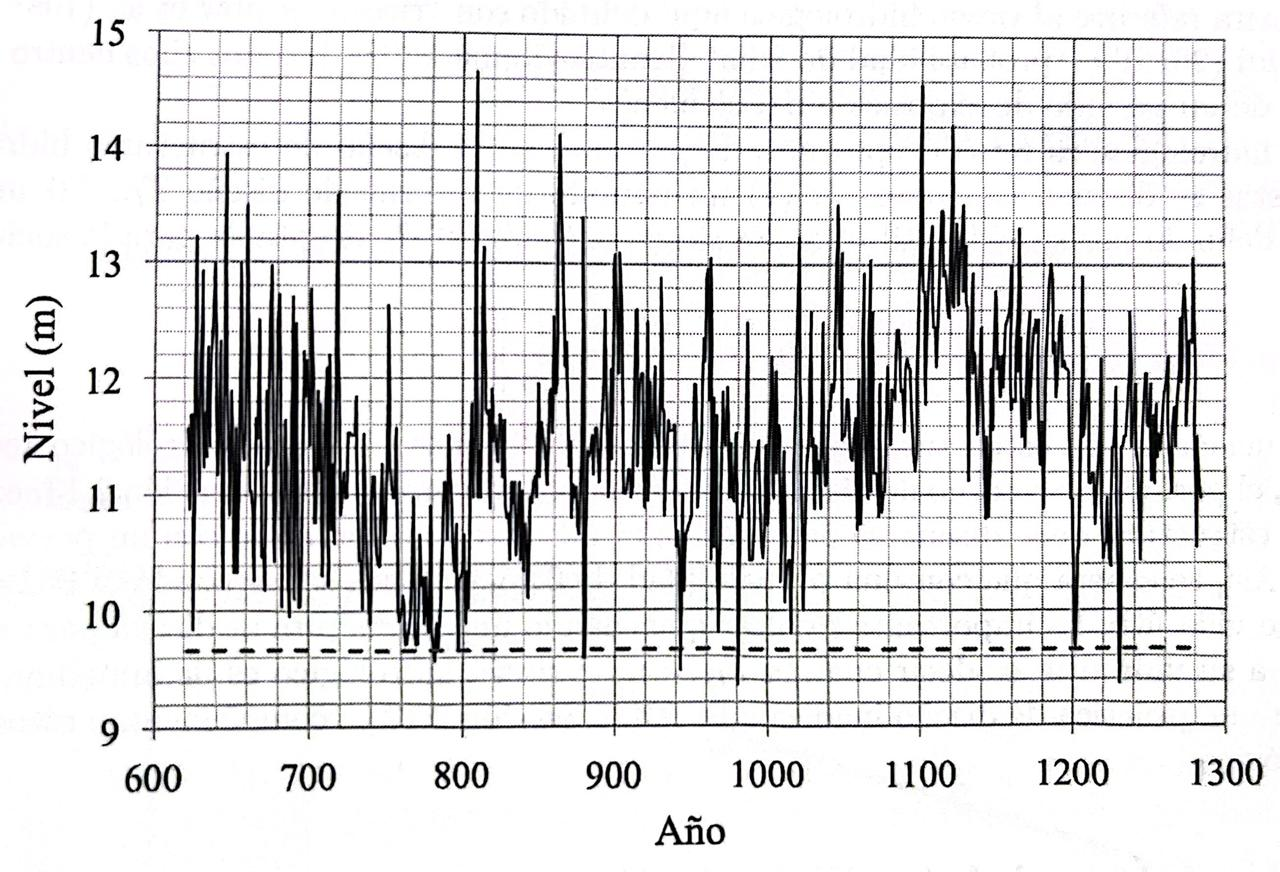
\includegraphics[width=1.2\linewidth]{fiM21.jpeg}  % from Diaz-Gra
\end{minipage}
\end{frame}

\begin{frame}{Return period}
    \begin{block}{Hydrological risk}
        According to the definition of risk, this involves the hazard of an certain elements. The \alert{hydrological risk} ($R_h$) is defined as the probability that the exposed element is affected by the hazard at least once during an exposure period  of $n$ years, that is:
        \[
            R_h = P[T \leq n] = 1-(1-p)^n
        \]
        Note that the hazard is defined by the probability $p = \frac{1}{T_R}$ and that $R_h$ is the complement of the probability that the exposed element is not  affected by the hazard during the exposure period of $n$ years, this means, it is the complement of $(1-p)^n$. The \emph{hydrological risk} is also known in the literature as the \alert{failure risk}.
        The \emph{hydrological risk} is important in the design of hydraulic structures because these are designed for a \emph{design period} ($T_D$) and a service life of $n$ years. Accordingly, $R_h$ can be written as:
        \[
            R_h = 1-\left( 1-\frac{1}{T_D} \right)^n
\]
For instance, an structure with a service life of 25 years and an acceptable hydrological risk of 15\%, the design period can be estimate from this equation and it is 154 years. It is expected that with a probability of 0.15, this could be surpassed at least once in the 25 years of service life. Note that is bad practice in design to make $T_D  = n$ because $R_h = 2/3$, which is quite high.
   \end{block}
\end{frame}

%-------
% From Diaz-granados
\section{Frequency analysis of extreme hydrological events}
\subsection{The purpose of the frequency analysis of extreme hydrological events}
\begin{frame}{The purpose of the frequency analysis of extreme hydrological events}
    The frequency analysis of extreme hydrological events seeks to estimate hazards and in particular to answer the following questions:
    \begin{itemize}
        \item What is the \emph{return period} of, for instance, a flood occurred in the XXXX year at the YY location where the water lever rise to ZZ m? 
        \item What the water level in the river XX at the YY location for a NN return period? This question can be considered as the inverse of the aforementioned question.
    \end{itemize}
    The frequency analysis can be shown graphically through the \alert{frequency curve}. An example of the frequency curve for the weekly average minimum streamflows are shown in the figure.

\centering
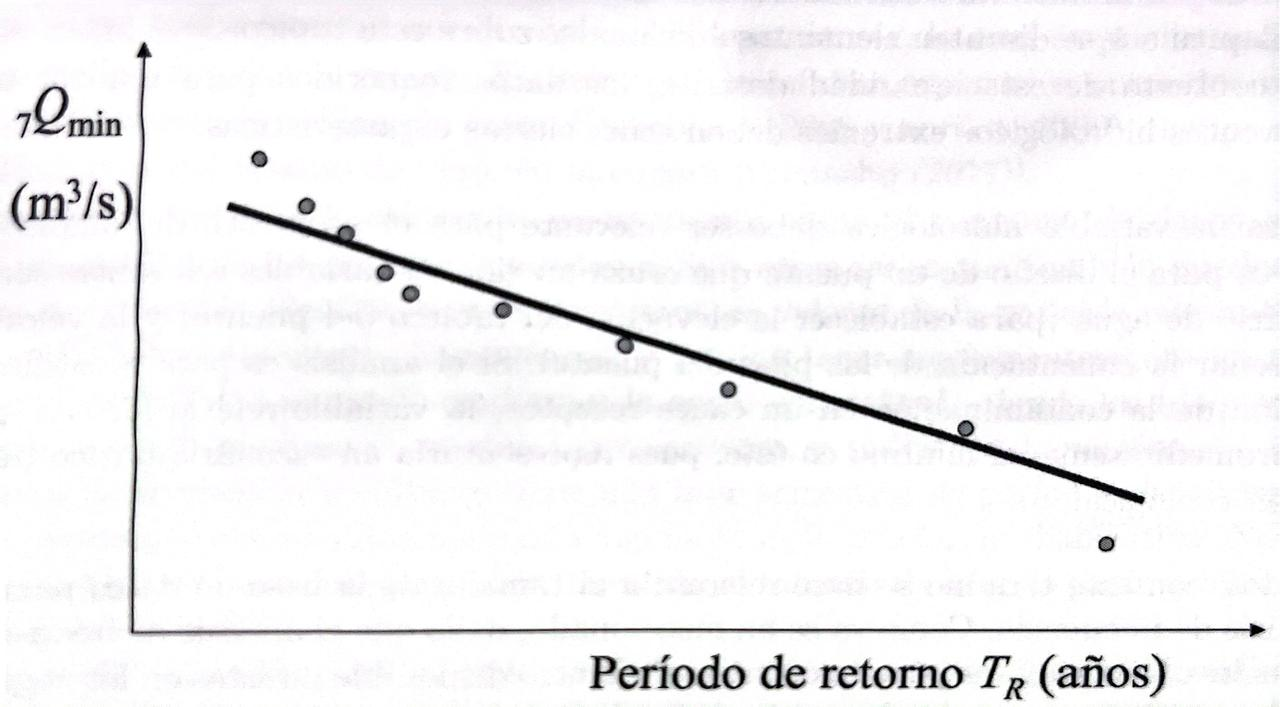
\includegraphics[width=0.95\linewidth]{fiM23.jpeg}  % from Diaz-Gra
\end{frame}

\subsection{The data needed for the analysis}
\begin{frame}{The data needed for the analysis}
The characteristics needed to the analysis of extreme hydrological events are described below:
\begin{itemize}
\item Use historical time series of records assuming that the data is \emph{stationary}, which means that the data \emph{pdf} does not change in time. Note that this assumption is partially denied because \emph{climate change} introduce non-stationary traits to the data (e.g. long term trends). 
\item The hydrological variable must be \emph{relevant} for the porpoise of the analysis. For instance, if an engineers is designing a bridge over a river, water level and flow speed are data needed for the design.   
\item The amount of data must be sufficient to the frequency analysis. As in the analysis of extreme events the number of data extracted from the data set is usually low, it is recommended to implement probability distribution with few parameters. These data must be \emph{independent and homogeneous} (from the same probability distribution). The minimum number of extreme values to perform an frequency analysis must be between 15 and 30. The larger the number the lesser the uncertainty in the estimation of the frequency curve.  
\item The data must come from the same gage in order avoid a mixing of errors. 
\item The data must represent or come from a homogeneous hydrological regime. This means that is not correct to mix within the same period, for instance, natural flows with regulated ones. 
\end{itemize}
\end{frame}

\begin{frame}{The data needed for the analysis}
    \begin{block}{Series}
    \alert{Series} are usually a time dependent sequence of data. From the series, the extreme data extracted can be classified as: 1) \emph{data blocks of maximum/minimum} and 2) \emph{maximum/minimum data over/under a certain threshold}. While the first type is extreme data extracted from a block (subset) of data, the second type is data that is over or under a predefined threshold. The most common first type data set is the \emph{annual series}. Annual series are formed after extracting the  maximum/minimum values of the raw time series for each year, where one year is one block. It is also needed to prove that the values extracted for each year are independent. This means that they must be separated enough in time so that no physical relationship (catchment time concentration) between values is possible.  An example of annual series is the maximum annual instantaneous discharge in a river gauge station. Semesterly series can also be formed when independence and homogeneity are guaranteed. In this case, the return period is estimated in semesters. Note that the smaller the block the larger the difficulty to guarantee independence and homogeneity. 
    In the case of the series formed after extracting maximum/minimum data over/under a certain threshold, the number of data per block can be greater than 1. For instance there must be more than one value of an specific year. Because is difficult to establish a return period from these series, this one serves to define a series of excess, that must be constituted by $n_y$ (number of years) values. In this series, the largest $n_y$ values are selected. In the case of \emph{bimodal} streamflow regimes, the semesterly series make sense, so the chosen of the block must obey the physical functioning of the natural system. 
    \end{block}
\end{frame}

\begin{frame}{The data needed for the analysis}
\centering
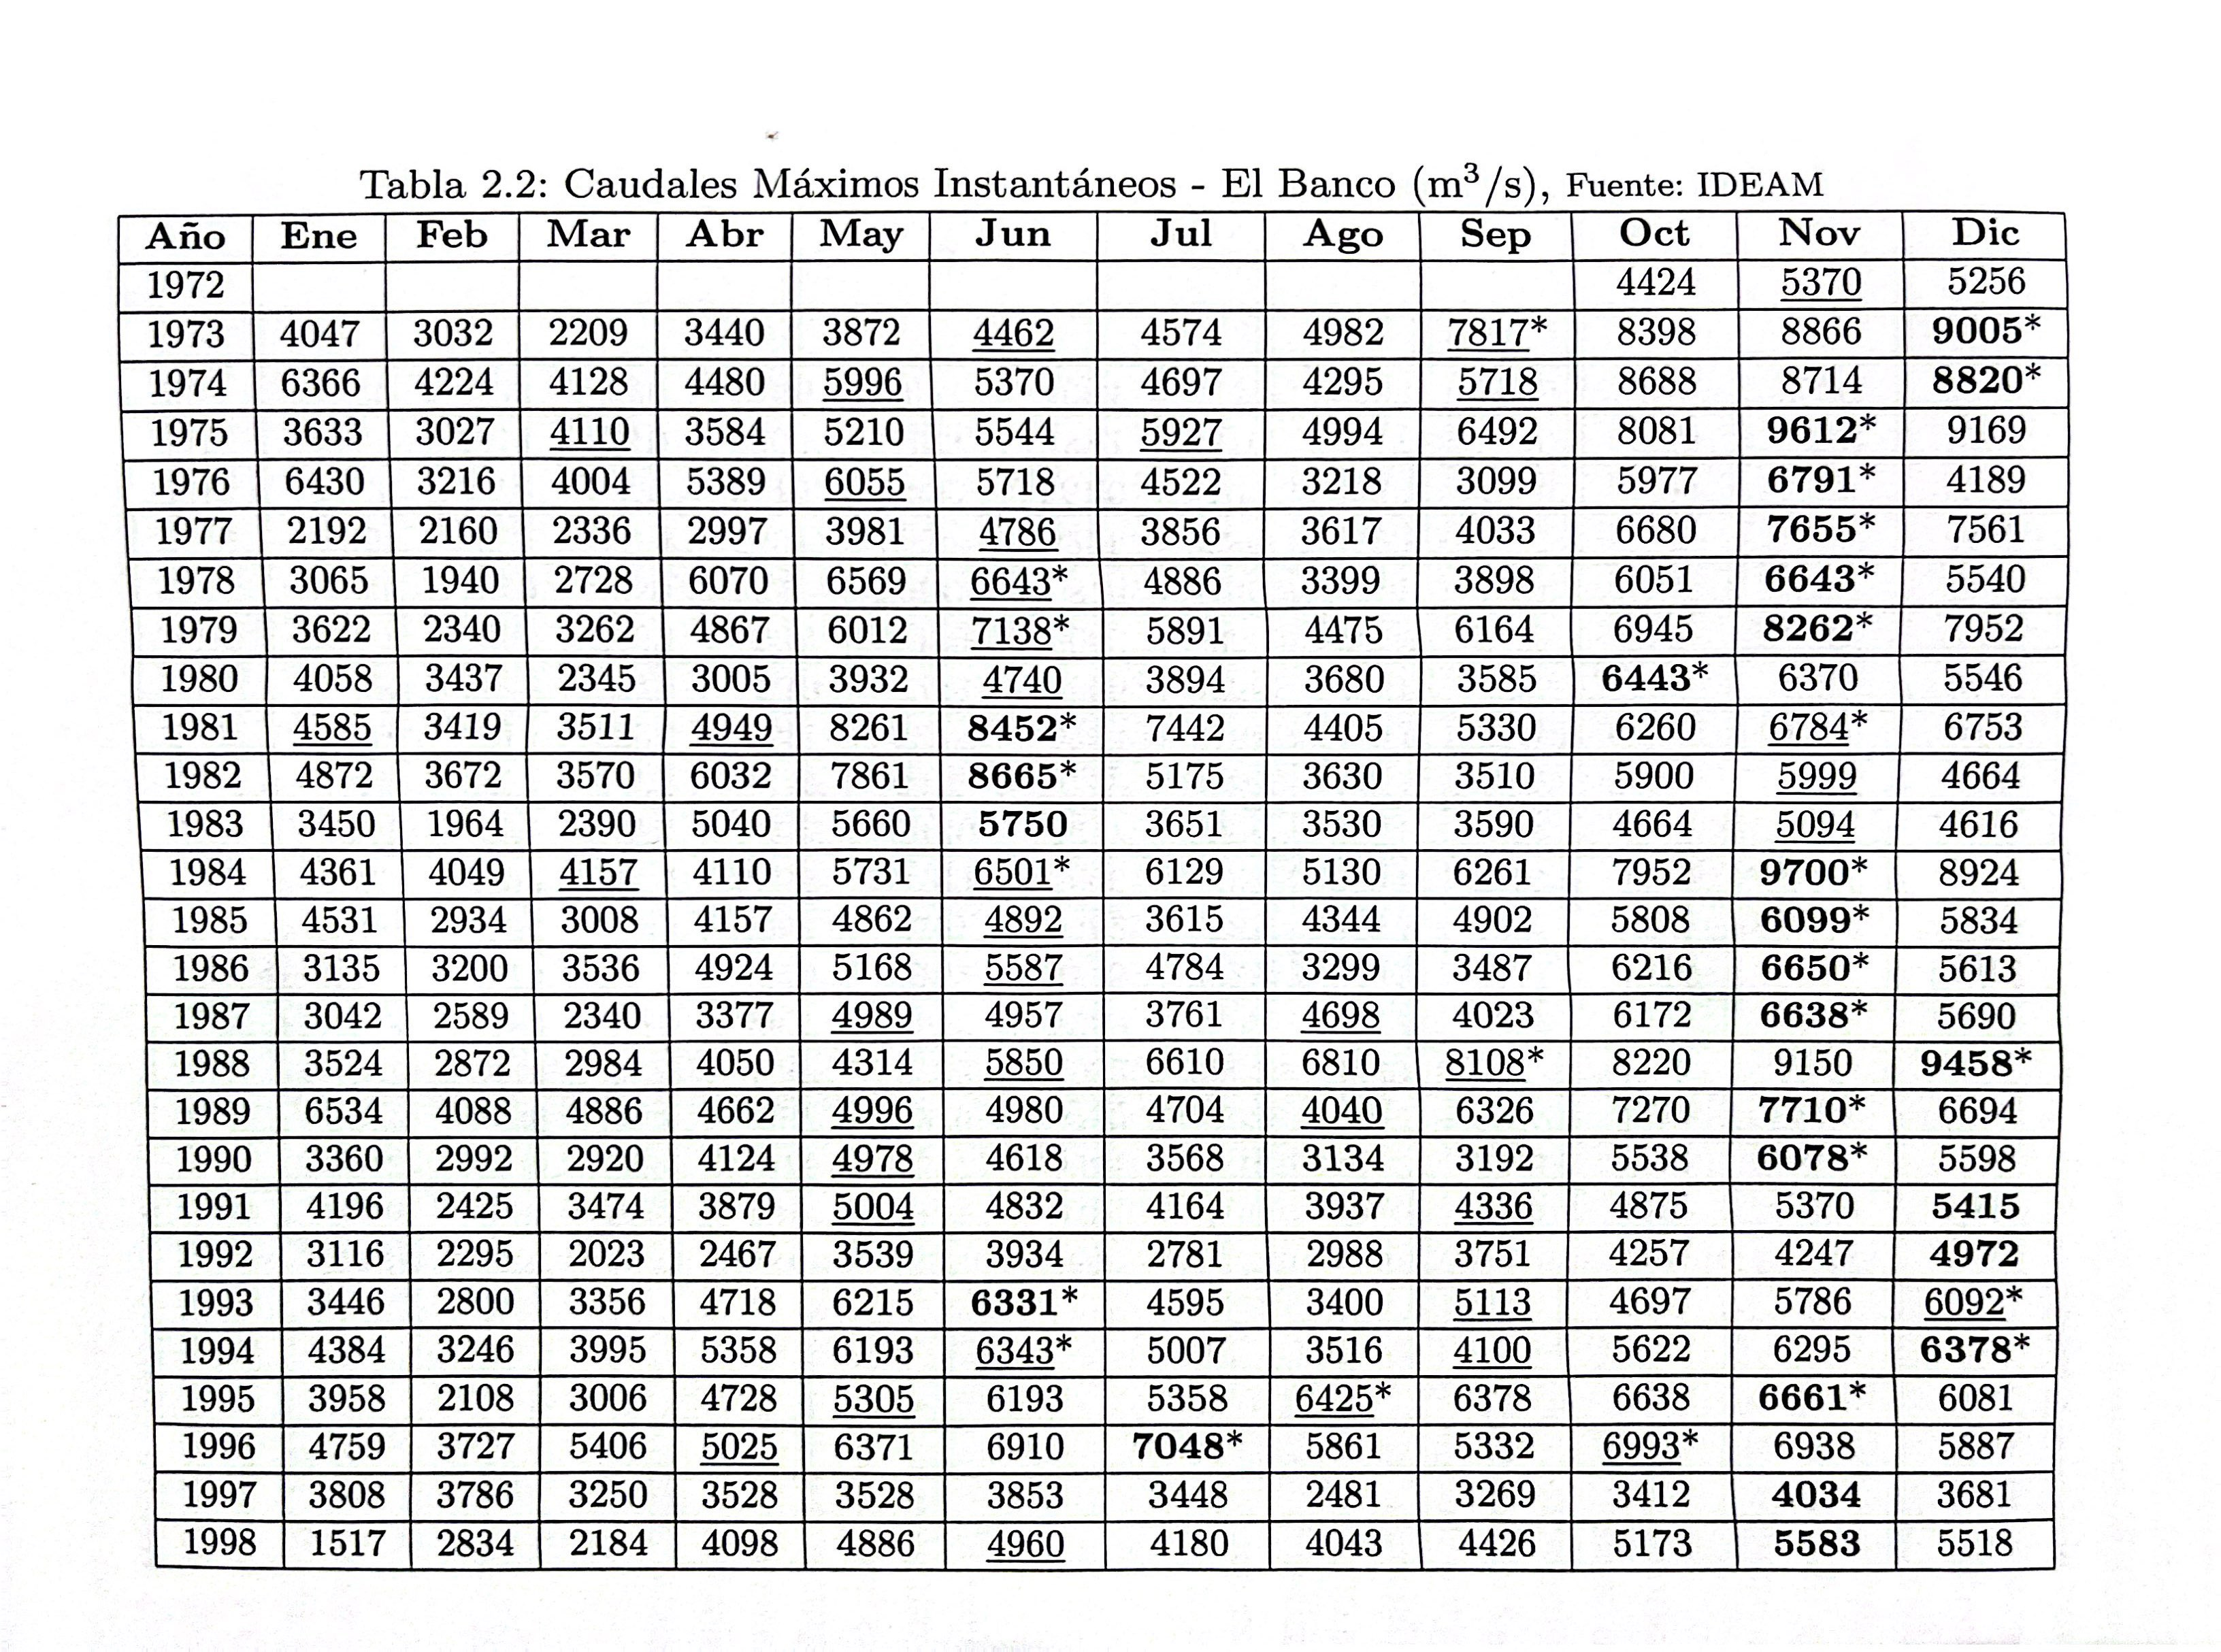
\includegraphics[width=\linewidth]{taM22.jpg}  % from Diaz-Gra
\end{frame}

\begin{frame}{The data needed for the analysis}
\centering
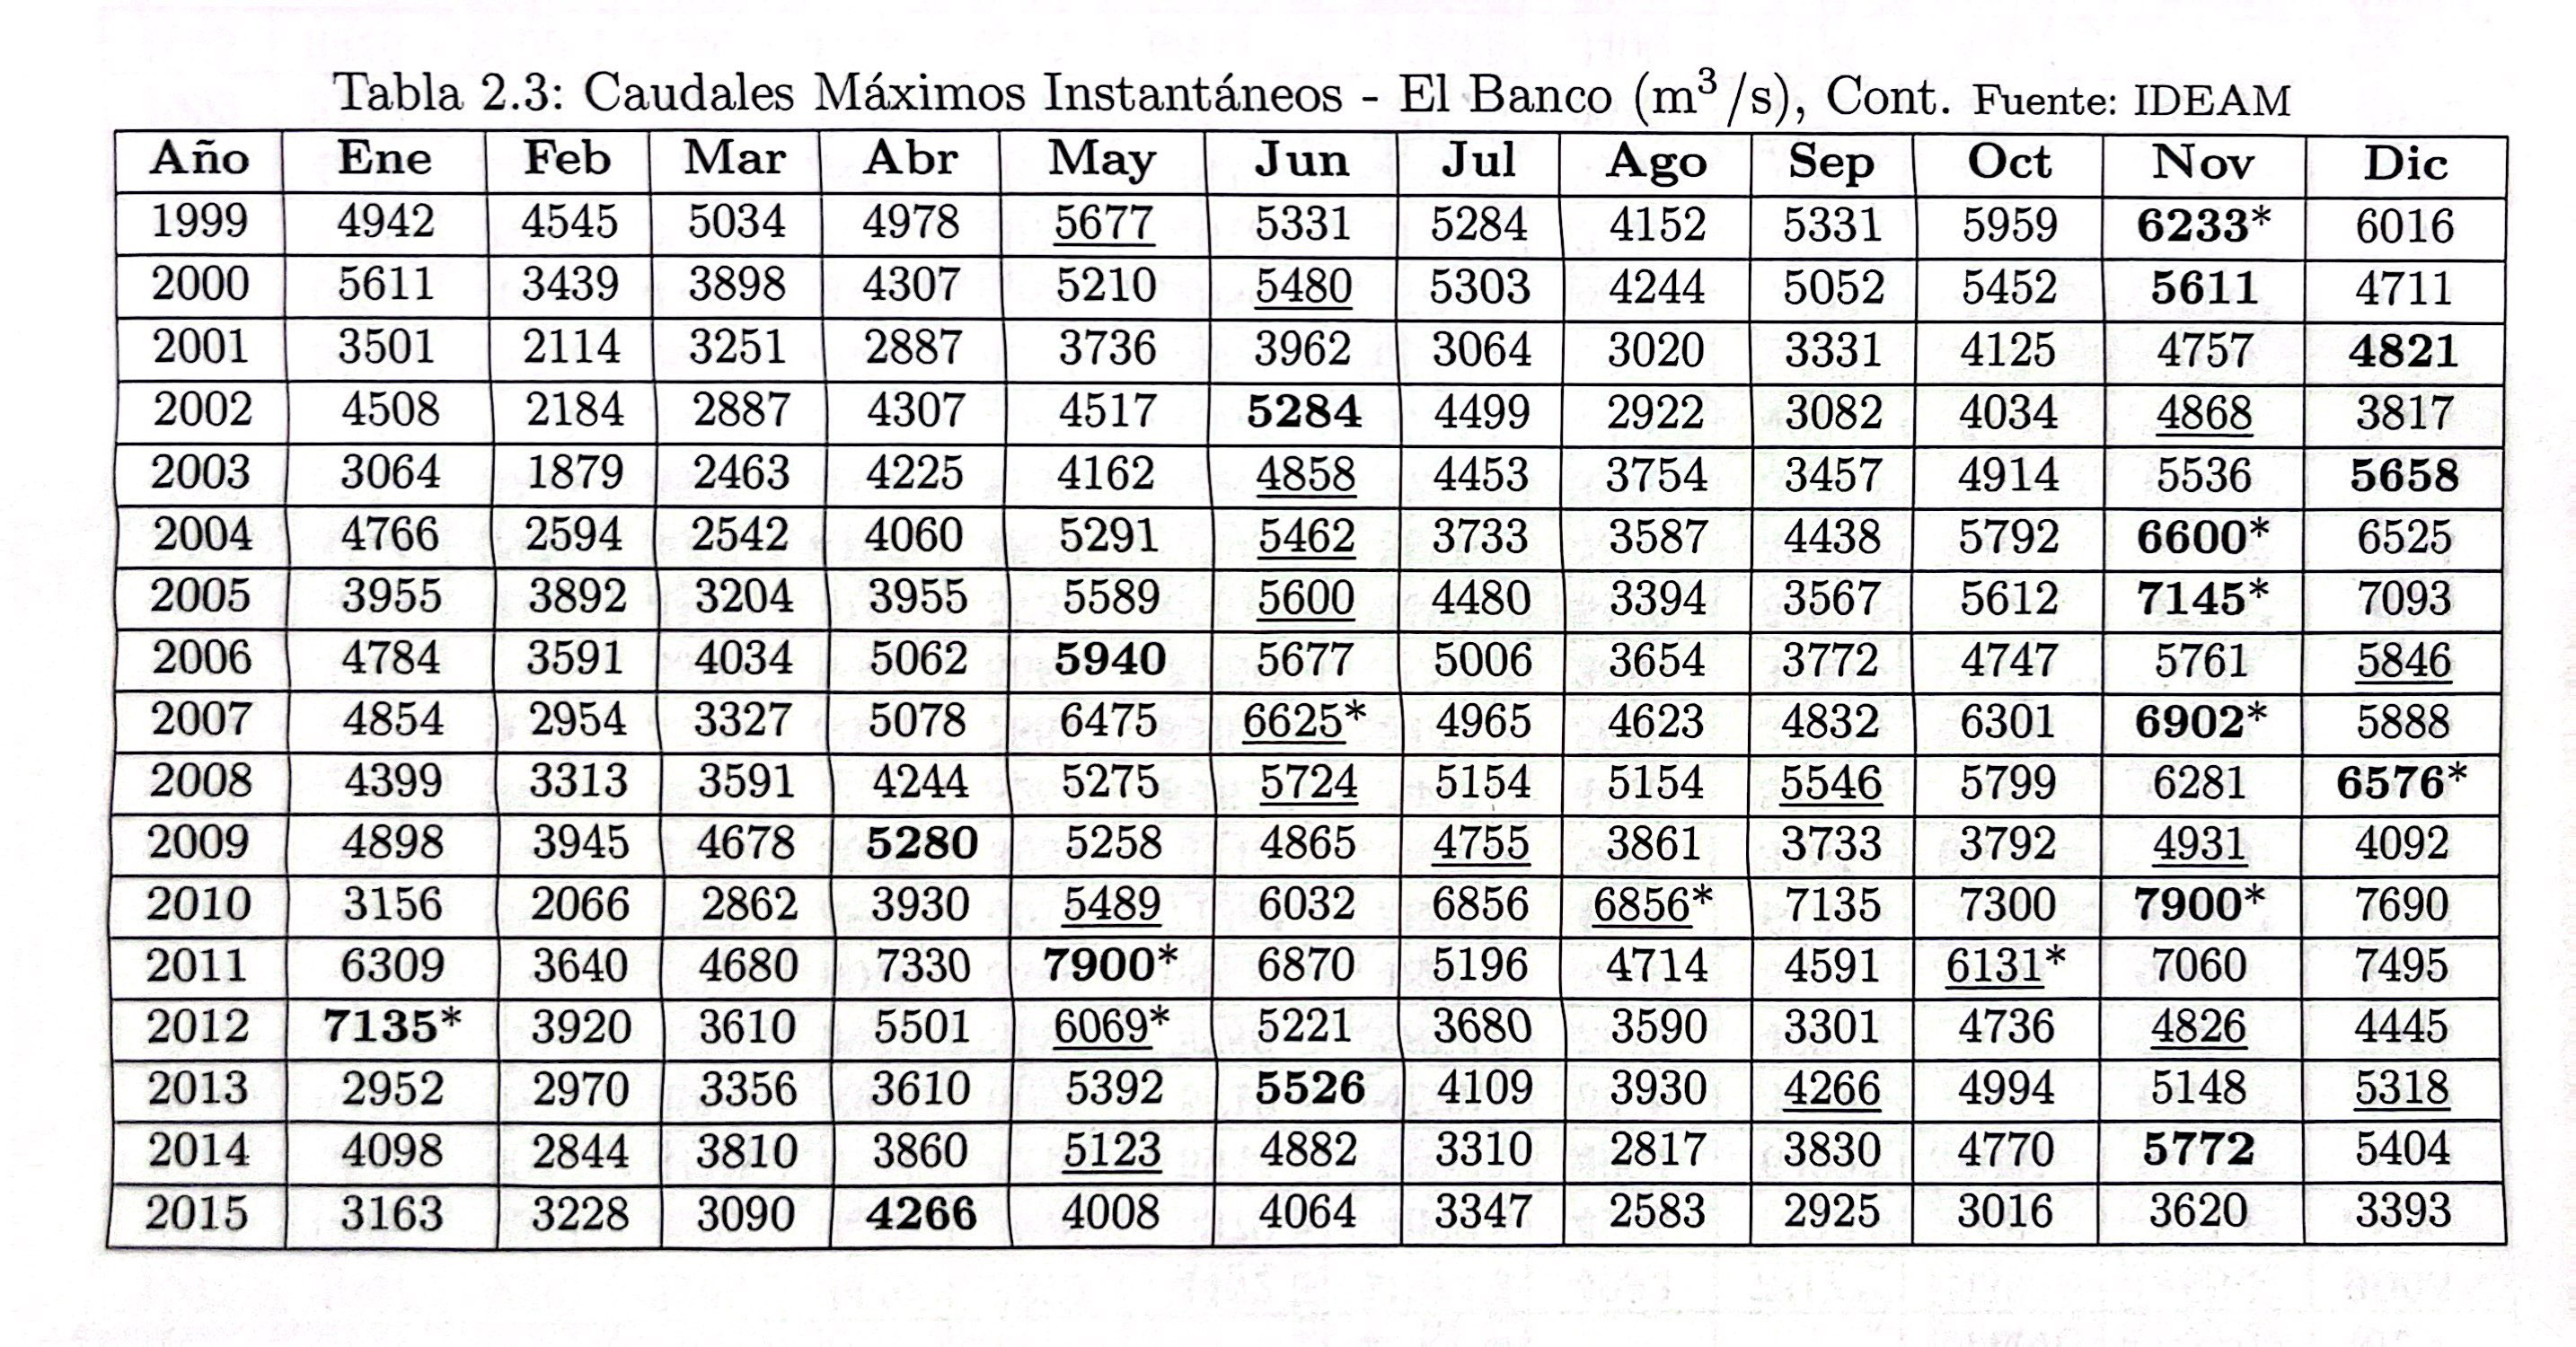
\includegraphics[width=\linewidth]{taM23.jpg}  % from Diaz-Gra
\end{frame}

\begin{frame}{The data needed for the analysis}
    \begin{block}{Hypothesis test for series}
        As we have told before data in any type of series must be \emph{independent and homogeneous}. The \emph{Kendall test} to verify that the data is stationary or not, check that whether $\mu$ is constant (\emph{null hypothesis} $H_0$)  or not (\emph{non null hypothesis} $H_1$). To apply the test is needed to estimate:
        \[
            S = \sum_{i=1}^{n-1} \sum_{j=i+1}^n sgn(x_j - x_i)
        \]
        where $x$ represent the hydrological variable, $sgn$ is the sign function where $sgn(a) = 1 \text{ if } a>0$, $sgn(a) = 0 \text{ if } a=0$ and $sgn(a) = -1 \text{ if } a<0$. Once $S$ is calculated, $K$ is calculated as:
 \[
K =
\begin{cases}
    \frac{S-1}{\sqrt{n(n-1) (2n+5)/18}}, & \text{for } S > 0  \\
     0 , & \text{for } S = 0  \\
    \frac{S+1}{\sqrt{n(n-1) (2n+5)/18}} & \text{for } S < 0
\end{cases}
\]
where $K$ follow a \emph{normal distribution} with $N(0,1)$. Accordingly, $H_0$ is accepted if $-z_{\alpha/2} \leq K \leq z_{-\alpha/2}$, where $z_{\alpha/2}$ is the value of $K$ that follow $N(0,1)$ which is exceeded with probability $\alpha/2$, where $\alpha$ is the significance. 
   \end{block}
\end{frame}


\subsection{Conceptual framework for  frequency analysis}
\begin{frame}{Conceptual framework for  frequency analysis}
    \begin{block}{Generalities}

        For a annual series is of interest to estimate the \emph{return period} ($T_R$) for a specific value $q$; for instance the $T_R$ for a extreme discharge occurred in a given year. As $T_R$ is the inverse of the probability $p$ that a value $q$ being equal or exceeded for maximum value series, and being equal or below for minimum value series, this means that $p$ must be estimated for a event of interest (minimum or maximum). There are different equations to estimate $p$ where the results among the equations are similar for short $T_R$ and they differ for long $T_R$. A general equation to estimate the probability $p$ is:
        \[
            p_i = \frac{i-0.439}{n+0.526}
        \]
        where $i$ is the order of data; maximum values are sorted in descending order and minimum values are sorted in ascending order. 
        It is also of interest to estimate the extreme value $q$ for a given $T_R$. This $T_R$ in many cases (e.g. $T_R = 100$ yrs) is larger than the time series length. For this, the data need to be fit to a probability distribution to extrapolate up to the $T_R$ of interest. To do this, for a series of annual maximum streamflows $Q$, note that $p = P[Q > q] = 1 - F_Q (q)$, where $F_Q (q)$ is the fitted \emph{cdf} of $Q$ annual extreme values. For a series of annual minimum streamflow $p = P[Q<q] = F_Q (q)$. 
   \end{block}
\end{frame}

\begin{frame}{Conceptual framework for  frequency analysis}
    \begin{block}{Probability distributions for the frequency analysis}
        Suppose a set of independent random variables $X_1, X_2, \cdots, X_n$  with a common \emph{cdf} $F_X (x)$, where $x$ is an observed value and $n$ is the number of values, usually, equally spaced, for instance, one year. Additionally, $X_{max} = max[X_1 , X_2 , \cdots, X_n ]$, and $F_{X_{max}} (x_{max})$ is given by the joint probability that $X_i \leq x_{max}$, that is:
        \begin{align*}
            P[X_{max} \leq x_{max}] &= P[X_1 \leq x_{max}, X_2 \leq x_{max}, \cdots, X_n \leq x_{max}] \\
                                    &=F_{X_1, X_2, \cdots, X_n} (x_{max}, x_{max},\cdots, x_{max})
        \end{align*}
        As $X_i$ are independent variables and follow the same probability distribution:
        \[
            F_{X_{max}} (x_{max}) = \prod_{k=1}^n P[X_k \leq x_{max} ] = \prod_{k=1}^n F_{X_k} (x_{max}) = \left[  F_{X} (x_{max}) \right]^n
        \]
        If $n \rightarrow \infty$ and if $X_{max}$ is standardized and converted into $Y$, the probability distribution must be one of the following types:
        \[
            \text{Type I:} \quad F_Y (y) = e^{-e^{-y}}, \text{ for } -\infty < y < \infty 
        \]
 \[
     \text{Type II: } F_Y (y) =
\begin{cases}
    &e^{-y^{-\gamma}} \text{ for } y > 0   \\
    &0 \text{ for } y \leq 0   \\
\end{cases}
\]
 \[
     \text{Type III: } F_Y (y) =
\begin{cases}
    &e^{-(-y)^{\gamma}} \text{ for } y < 0   \\
    &1 \text{ for } y \geq 0   \\
\end{cases}
\]
  \end{block}
\end{frame}

\begin{frame}{Conceptual framework for  frequency analysis}
    \begin{block}{Probability distributions for the frequency analysis}
        This types can be the following probability distributions:
        \begin{itemize}
            \item \emph{Type I:} Exponential, Gamma, Weibull, Normal, Lognormal, Logistic and Gumbel type I.
            \item \emph{Type II:} Pareto, t-student, Cauchy, Loggamma, Frechet type II
            \item \emph{Type III:} Uniform, Beta, Weibull type III.
        \end{itemize}
        Note that the \emph{type I} distributions are not bounded and do not serve to represent maximum and minimum values, while the \emph{type II} distribution are bounded in the inferior limit and are suitable to fit maximum values. In the case of \emph{type III} distributions, these are bounded in the superior limit and are suitable for minimum values. 
 Some of these distribution converge slowly to the limit distribution and are thus unsuitable for the analysis of extreme events. In consequence, there are other distributions or modifications to some of the distributions mentioned that can be implemented for the analysis of extremes. 
  \end{block}
\end{frame}

\begin{frame}{Conceptual framework for  frequency analysis}
    \begin{block}{Frequency equation}
        The \alert{frequency equation} is given by:
        \[
            x_T = \mu_X + K_T \sigma_X
        \] 
        where $x_T$ is the magnitude of the event with a return period $T$, $\mu_X$ and $\sigma_X$ are the mean and the standard deviation of the distribution, respectively, and $K_T$ are the \alert{frequency factor} that depends of the return period and the specific probability distribution. The equations to estimate the frequency factor are found probability textbooks. Note that $\mu_X$ and $\sigma_X$ need to be estimated based in the \emph{pdf} parameters estimated based on the annual series.

 \end{block}
\end{frame}

\begin{frame}{Conceptual framework for  frequency analysis}
    \begin{block}{Estimation of the confidence limits}
        It is important to point out that the magnitude $x_T$ of the extreme event with a return period $T$ is a random variable that follow a \emph{pdf}. For an   ascending sorted annual series $x_{1:n} \leq x_{2:n} \leq \cdots \leq x_{n:n}$, the \emph{pdf} of $X_{k:n}$ is:
        \[
            f_{X_{k:n}} (x) = \left( \begin{array}{c} n \\ k \end{array} \right) (k)  \left[ F_X (x) \right]^{k-1} \left[ 1 - F_X (x) \right]^{n-k} f_X (x)
            \]
            where $f_X (x)$ and $F_X (x)$ are the fitted \emph{pdf} and \emph{cdf}, respectively, based on the annual series. Note that the \emph{pdf} of $X_{k:n}$ has the same characteristics of the \emph{pdf} fitted to the annual series and a position of order $k$. Accordingly, the \emph{fdp} of $X_T$ is:
        \[
            f_{X_T } (x_T) = \left( \begin{array}{c} n \\ m \end{array} \right) (m)  \left[ F_X (x_T) \right]^{m-1} \left[ 1 - F_X (x_T) \right]^{n-m} f_X (x_T)
            \]
            where $m$ is the integer fraction of $nr$ and $r = 1 -\frac{1}{T}$. So if $f_{X_T} (x_T)$ is known, the confidence limits can be estimated. For instance, to the 90\% of confidence, the inferior and the superior limits must satisfy  that $F_{X_T} (x_{T_inf}) = 0.05$ and $F_{X_T} (x_{T_sup}) = 0.95$.                 
\end{block}

\end{frame}

\begin{frame}{Conceptual framework for  frequency analysis}
        \vspace{-5pt}
    \begin{block}{Estimation of the confidence limits} 
        These \emph{pdf} equations correspond to the \emph{Beta distribution}. This is actually the incomplete Beta function standardized by the Beta function. The exact confidence intervals can be estimated numerically solving this equations:
        \vspace{-8pt}
            \begin{align*}
                I[P; n' P_{inf}, n' (1-P_{inf})] &= 1-\alpha/2 \\
                I[P; n' P_{sup}, n' (1-P_{sup})] &= \alpha/2 \\
            \end{align*}
        \vspace{-8pt}
            where:
        \vspace{-8pt}
            \[
                I(z; a,b) = \frac{\Gamma(a + b)}{\Gamma(a+1) \Gamma (b)} z^a (1-z)^b + \frac{\Gamma(a + b + 1)}{\Gamma(a+1) \Gamma (b)} \int_0^z t^a (1-t)^{b-1} dt
            \]
            and $n' = (n+1)$. Note that int the equation for $I[]$, $z = P$, $a = n' P_{inf}$ or $a = n' P_{sup}$, and $b = n' (1-P_{inf})$ or $b = n' (1-P_{sup})$. The problems is to find the values of $a$ and $b$ using the two equations for a given value of $\alpha$ $P$. Suppose that one want to estimate the confidence limits for a 90\% confidence for the value from the frequency curve that correspond to a return period of $T=50$ years. The equations above are solved for $\alpha = 1-0.9 = 0.1$ and $P = 1 - \frac{1}{T} = 1- 1/50 = 0.98$.
            Note that traditionally, the confidence limits for $x_T$ have estimated assuming that $X_T$ follow a \emph{Normal distribution}, so the confidence limits can be estimated approximately as:
        \vspace{-12pt}
            \begin{align*}
                x_{T_{inf}} &= x_T - z_{\alpha/2} s_T \\
                x_{T_{sup}} &= x_T + z_{\alpha/2} s_T 
            \end{align*}
            where $\alpha$ is the level of significance, $z_{\alpha/2}$ is the value of the standardized variable which is exceeded with probability $\alpha/2$, and $s_T$ is the estimate of the standard deviation of the event with a return period $T$. Note that $s_T$ is usually estimated using the Moments or the Maximum-likelihood methods.
\end{block}

\end{frame}

\begin{frame}{Conceptual framework for  frequency analysis}
 \begin{exampleblock}{Confidence limits of return period} % from Diaz-Gra
     The exact confidence limits for the 90\% of confidence of the frequency curve of instantaneous maximum streamflows for the Banco station at the Magdalena river (see the tables with data given before) are shown in the table below:

     \begin{center}
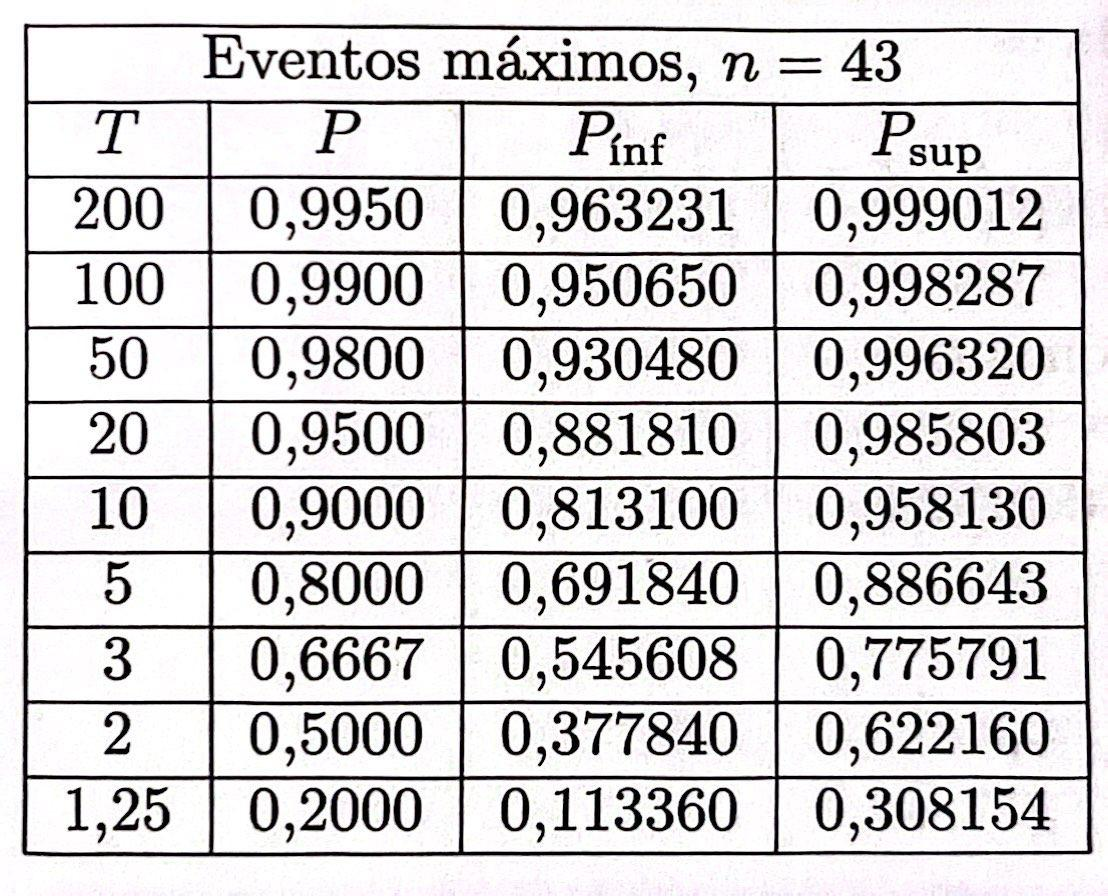
\includegraphics[width=0.5\linewidth]{taM26.jpeg}  % from Diaz-Gra
     \end{center}

     Note that the equations given before are solved for: $n=43$ (\# of years), $\alpha = 0.1$, and various values of $T$. The equations are solved to find the values for $P_{inf}$ and $P_{sup}$ given in the table. The confidence limits can then be estimated using the fitted \emph{cdf} as $x_{T_{inf}} = F^{-1} (P_{inf})$ and $x_{T_{sup}} = F^{-1} (P_{sup})$.
 \end{exampleblock}

\end{frame}






\end{document}

